\chapter{Error propagation matrices}

\section{Space variant propagation matrix}

\label{sec:convolution_kernels}

\label{sec:kernels}
When using a space-invariant convolution kernel $W = W_{\vec p}$, the minimum error search presented in section \ref{sec:minimum_error_search} implies that it is possible for pixels belonging to objects other than the object at the center pixel $\vec p$ to influence the accumulated error value. A mechanism that restricts the error propagation to regions belonging to the same object is desirable.

The assumption made here is that different objects (with possibly different depths) in the scene are separated by visible edges. This assumption appears to be reasonable, as the absence of edges in the input image means that the scene consists of homogeneously colored surfaces. In that case, it would not be possible to reconstruct depth at all.

Note that the inverse of the assumption does not hold: Objects might have inner edges that do not imply any change in depth. Yet this should be unproblematic as the presence of structured surfaces allows for distinct minimums in the error stack and thus a higher quality depth reconstruction.

Let $\img{CV_{E}}(\vec p)$ denote the edge amplitude of the current view image where $\vec p = (x, y)^T$:
	$$\img{CV_{E}}(\vec p) = \sqrt{\left(\left.\frac{\partial \img{CV}}{\partial x}\right|_{\vec p}\right)^2 + \left(\left.\frac{\partial \img{CV}}{\partial y}\right|_{\vec p}\right)^2}$$
The entries $w_{ij}$ in the $2r_W + 1 \times 2 r_W + 1$ filter kernels $W_{\vec p}$ (with $i, j \in \{-r_W, \ldots, r_W\}$) specify how many edges are located between the center pixel $\vec p$ and the position referenced by $i, j$. This way only the error values of pixels that are not separated from the center pixel by edges will be propagated. Let $w_{ij}'$ denote the unnormalized error propagation matrix entires:
\begin{equation}
	w_{ij}' = \prod_{\tilde p \in \mathrm{Path}(\vec p, \vec p + (i, j)^T)} (1 - \img{CV_{E}}(\tilde p)) \label{eqn:error_matrix_bresenham}
\end{equation}
Where $\mathrm{Path}(\vec p_1, \vec p_2) : \R^2 \times \R^2 \longrightarrow \mathcal{P}(\R^2)$ returns a set of points that lie on the line between $\vec p_1$ and $\vec p_2$. Such a set can for example be calculated using Bresenham's line algorithm (see \cite{bresenham}).

A less sophisticated approximation is given by following the principal axes in the matrix instead of straight paths. This results in the following formula:
\begin{equation}
	w_{ij}' = \left( \prod_{\tilde \imath \in \{0, \ldots, i\}} (1 - \img{CV_{E}}(x + \tilde \imath, y + j)) \right) \cdot \left( \prod_{\tilde \jmath \in \{0, \ldots, j\}} (1 - \img{CV_{E}}(x + i, y + \tilde \jmath)) \right)
	\label{eqn:error_matrix_approx}
\end{equation}
A visualization of the propagation matrix calculation process can be found in figure \ref{fig:error_propagation}. In the experiments this significantly faster, second method is used.

\begin{figure}[tb]
	\begin{center}
		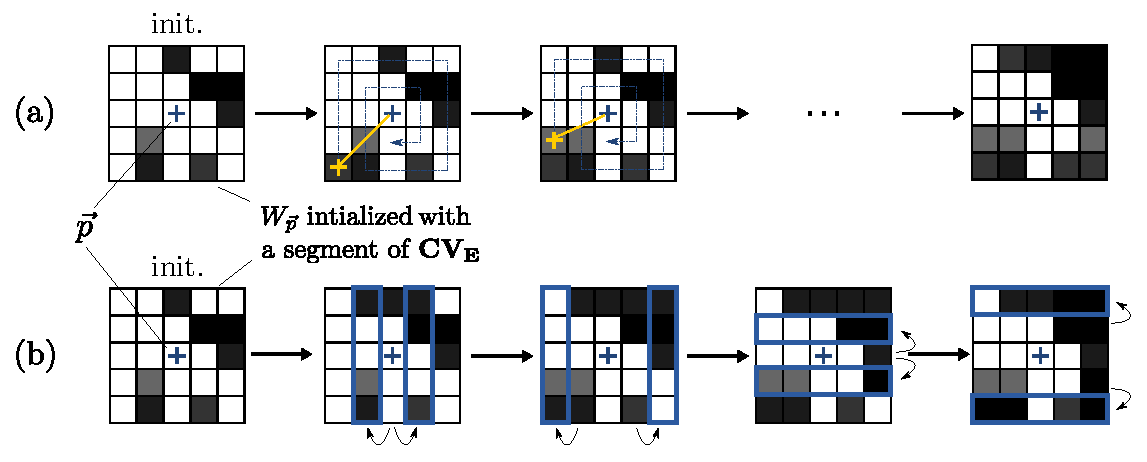
\includegraphics[scale=0.65]{media/error_propagation.pdf}
	\end{center}
	\caption{Step-by-step visualization of the error propagation matrix calculation. The top figure (a) visualizes the calculation as given in equation \ref{eqn:error_matrix_bresenham}, (b) shows the calculation resulting from the approximation in equation \ref{eqn:error_matrix_approx}. In (a) the values from the edge image (black pixels correspond to edges) are multiplied along a line starting from the center pixel $\vec p$ (blue) to the target pixel (yellow). Choosing the target pixels along a spiral path allows the matrix to be updated in-place. The approximation in (b) can be calculated by in-place multiplication of neighboring columns and rows respectively starting from the center.}
	\label{fig:error_propagation}
\end{figure}

The entries of the normalized propagation matrix are given as
\begin{equation*}
	w_{ij} = \frac{w_{ij}'}{\sum_{i, j} w_{ij}'}
\end{equation*}

\section{Propagation matrix performance}

\begin{figure}[t]
\begin{center}
 \textbf{Apartment scene}\\
 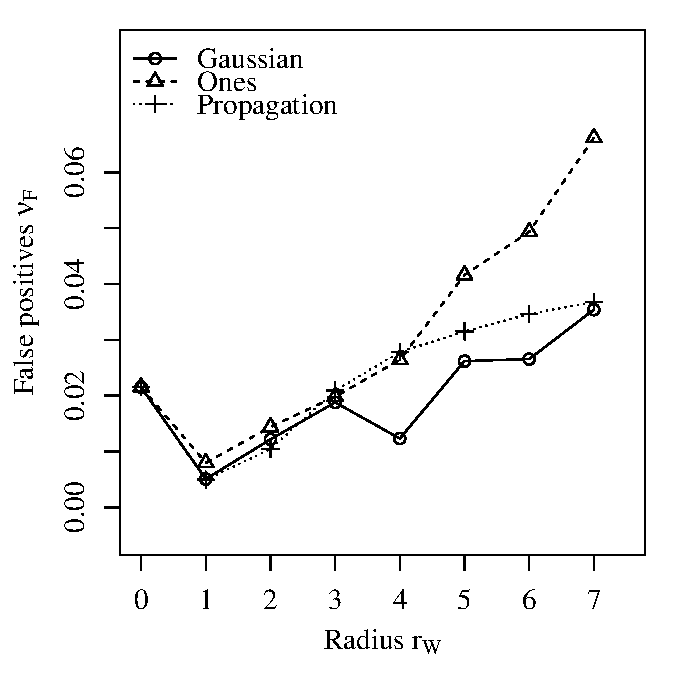
\includegraphics[width=0.475\textwidth]{results/matrices/propmat_apartment_mF.pdf}
 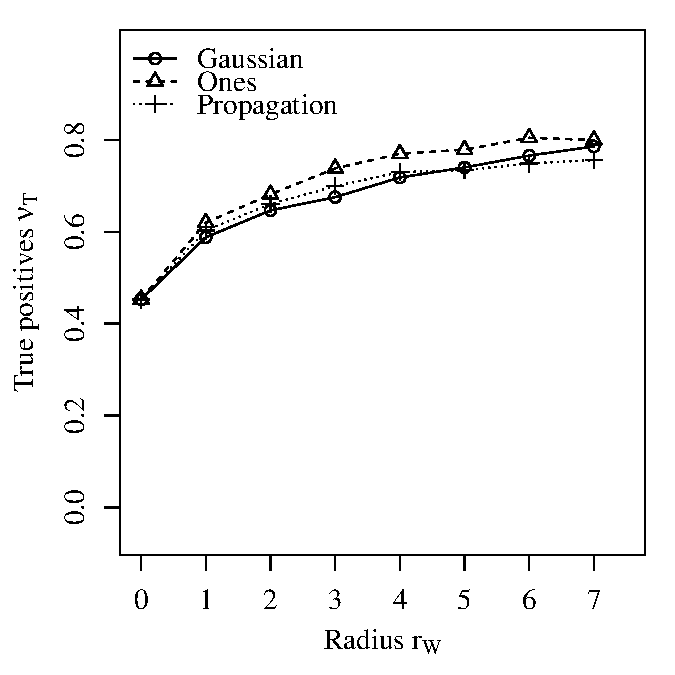
\includegraphics[width=0.475\textwidth]{results/matrices/propmat_apartment_mT.pdf}
 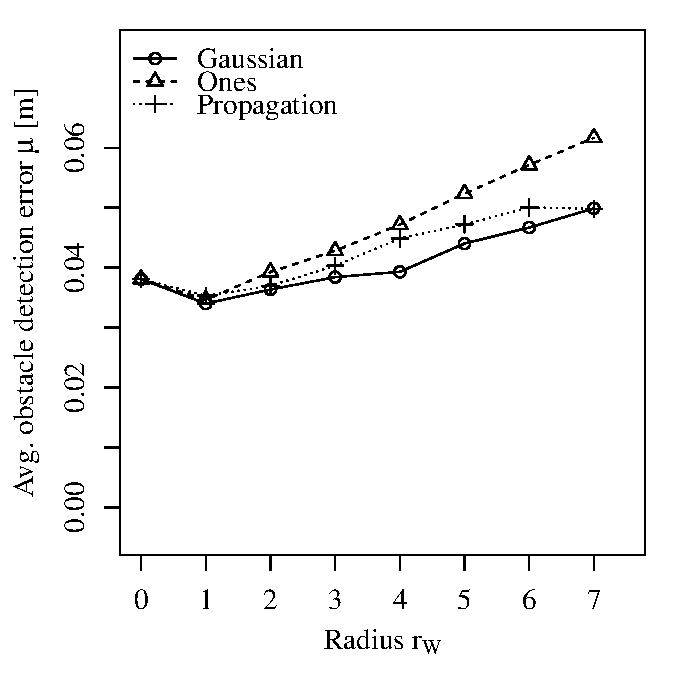
\includegraphics[width=0.475\textwidth]{results/matrices/propmat_apartment_meanDist.pdf}
 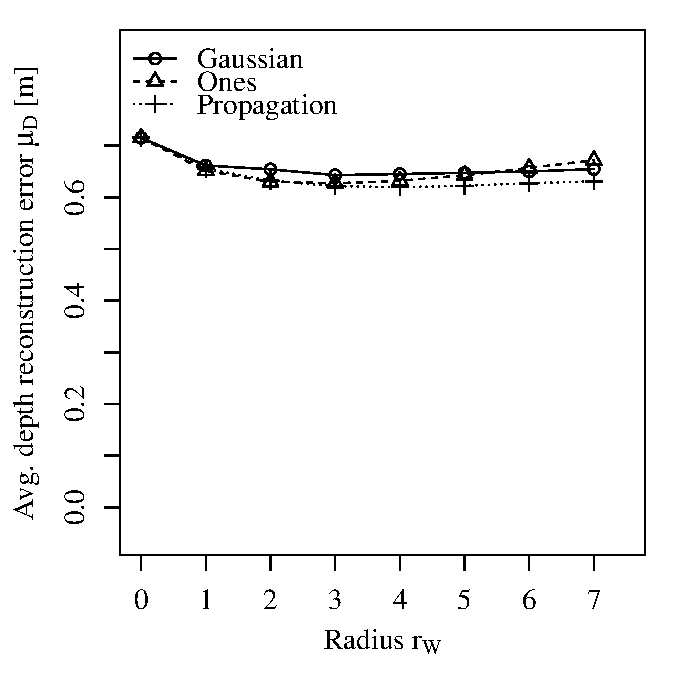
\includegraphics[width=0.475\textwidth]{results/matrices/propmat_apartment_avgNettoMean.pdf}
\end{center}
\caption{Results for varying propagation matrices $W_{\vec p}$ in the apartment scene.}
\label{fig:results_propagation_apa}
\end{figure}

\begin{figure}[t]
\begin{center}
 \textbf{Laboratory scene}\\
 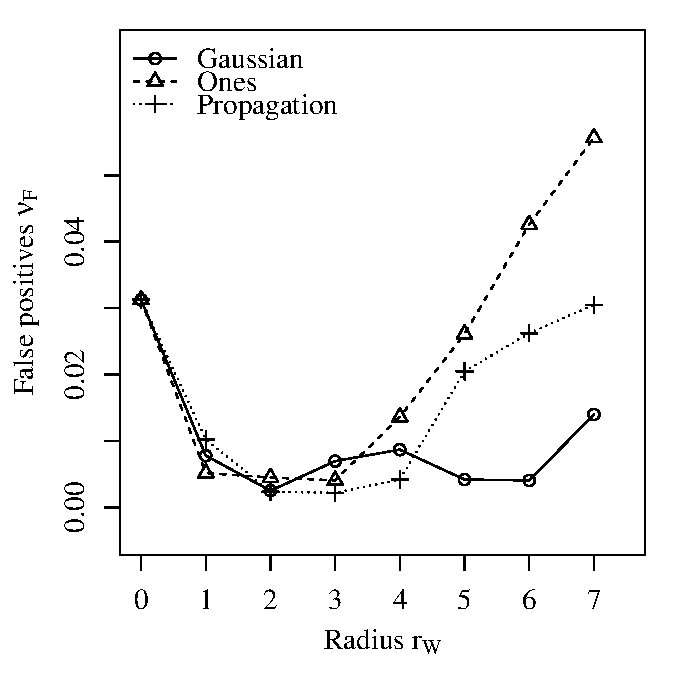
\includegraphics[width=0.475\textwidth]{results/matrices/propmat_laboratory_mF.pdf}
 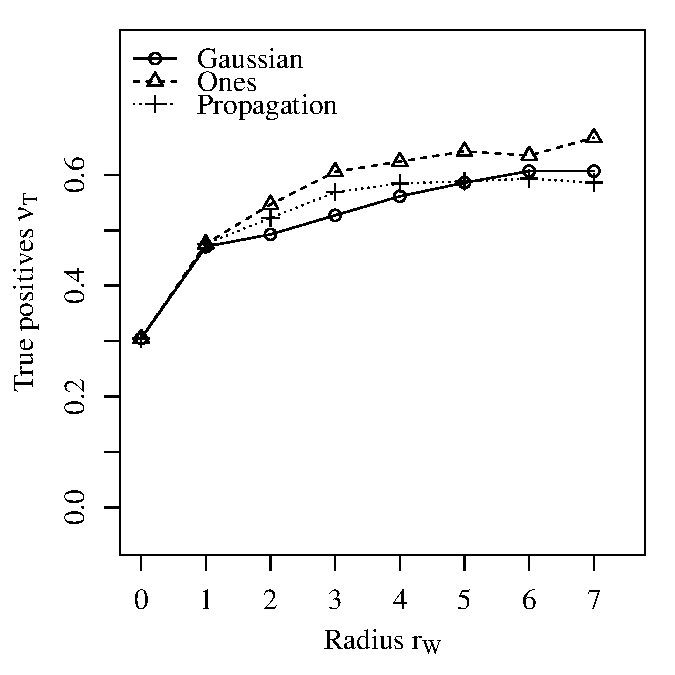
\includegraphics[width=0.475\textwidth]{results/matrices/propmat_laboratory_mT.pdf}
 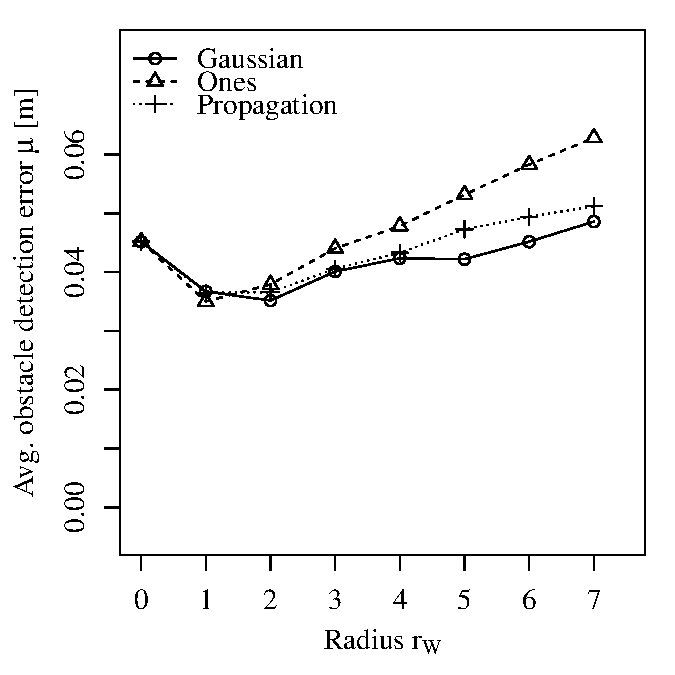
\includegraphics[width=0.475\textwidth]{results/matrices/propmat_laboratory_meanDist.pdf}
 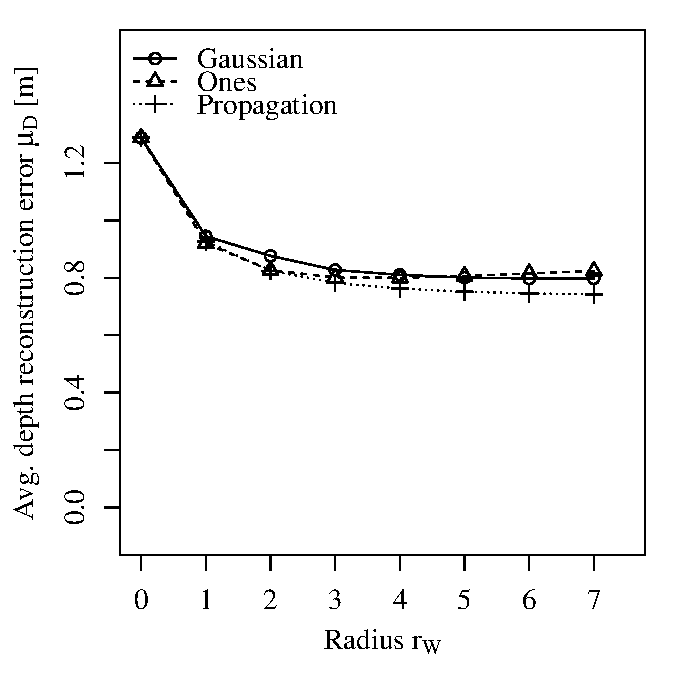
\includegraphics[width=0.475\textwidth]{results/matrices/propmat_laboratory_avgNettoMean.pdf}
\end{center}
\caption{Results for varying propagation matrices $W_{\vec p}$ in the laboratory scene.}
\label{fig:results_propagation_lab}
\end{figure}

\label{sec:results_propagation}

\paragraph{Experiment description:} The tests in this section are performed in order to determine the best type and radius $r_W$ of the error propagation matrix $W_\vec{p}$. Note that this test is performed using the (non-realtime) author's personal reference implementation (not described in this thesis), as support for different types of error propagation matrices and varying radii was removed from the optimized implementation.

The experiment is conducted in the simulated environments described in section \ref{sec:experiments}. In the test both the propagation matrix radius $m \in \{0, \ldots, 7\}$ and its type are varied. The types include a discrete Gaussian filter kernel (approximated using a binomial filter kernel, dubbed ``Gaussian''), a box filter (matrix of ones, dubbed ``Ones''), and the error propagation matrix as described above (dubbed ``Propagation'').

\paragraph{Results:} The results of the this experiment can be seen in figures \ref{fig:results_propagation_apa} and \ref{fig:results_propagation_lab}. One can see that for $r_W > 0$ the relative count of false positives $\nu_F$ first decreases but increases again for larger $r_W$. The same is true for the average obstacle detection error $\mu$. The relative count of true positives $\nu_T$ increases with increasing $r_W$. An extraordinarily high increase in $\nu_T$ and (along with a large drop in $\nu_F$ and $\mu_D$) can be seen in the step from $r_W = 0$ to $r_W = 1$).

Generally speaking there is no large difference in the performance of the different propagation matrix types. Yet the ``Ones''-matrix tendentially shows the worst performance and the ``Propagation''-matrices have a slightly superior depth reconstruction performance for large $r_W$.

A $3 \times 3$ (radius $r_W = 1$) binomial filter kernel was chosen for the optimized implementation: Larger radii increase the run time and do not necessarily yield a higher obstacle detection quality. The propagation matrices described above were not used, as they introduce an additional calculation step and (in contrast to the binomial kernel) are not separable and not space-invariant.
